\documentclass[14pt]{article}

\usepackage[polish]{babel}
\usepackage[utf8]{inputenc}
\usepackage[T1]{fontenc}
\usepackage{extsizes}
\usepackage{graphicx}
\usepackage{tocloft}
\usepackage{amsmath}
\usepackage{multirow}
\usepackage{hyperref}


\font\titlefont=cmtt10 at 22pt

\title{
    
\includegraphics[scale=0.5]{images/logo-pwr-pion.png}
    \vspace{1cm}
    \\
    {\textbf{
    \titlefont Sygnały i obrazy cyfrowe
    \\ Laboratorium 5 - Depoissoning
    }}
}
    
\author{
    Informatyczne Systemy Automatyki
    \\
    \\ Wykonujący:
    \\ Igor Potyrała - 272518
    \\
    \\ Prowadzący - Przemysław Śliwiński
}
\date{Data laboratoriów: 20 grudnia 2023}


\begin{document}
\maketitle
\newpage
% Spis treści
%\newpage
%\renewcommand{\cftsecleader}{\cftdotfill{\cftdotsep}}
%{
 % \hypersetup{linkcolor=black, hidelinks}
 % \tableofcontents
%}

% Wstęp teoretyczny, definicje
\section{Zadania}
\subsection{Cel zajęć}
Zadanie polega na porównaniu jakości 
interpolacji obrazów podczas 
filtrowania ich z szumów i wygładzania.


\subsection{Wyniki}
\vspace{1cm}
\begin{center}
    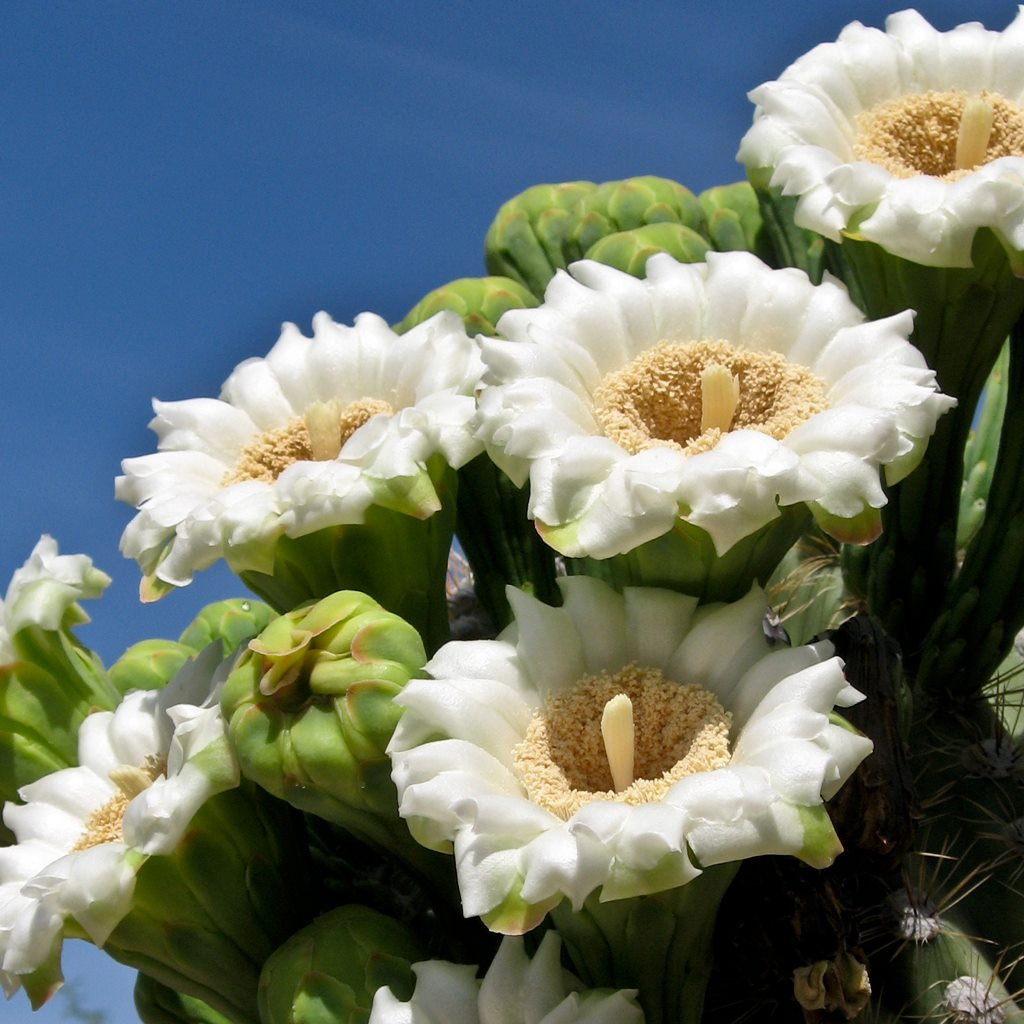
\includegraphics[scale=0.15]{images/cactus.jpg}
    \\ \small Obraz 1. Oryginalny obraz.

    % k = 1
    %\vspace{0.5cm}
    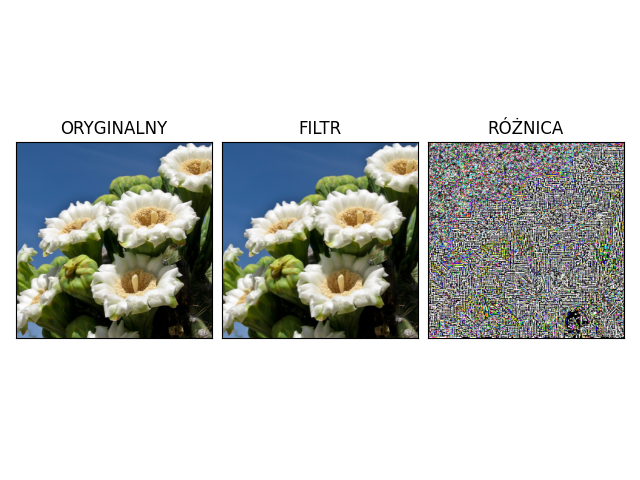
\includegraphics[scale=0.7]{images/nn_k1_p7.png}
    \\ \small Obraz 2. po interpolacji najbliższego sąsiada, 
    $k=1$, $p=7$.

    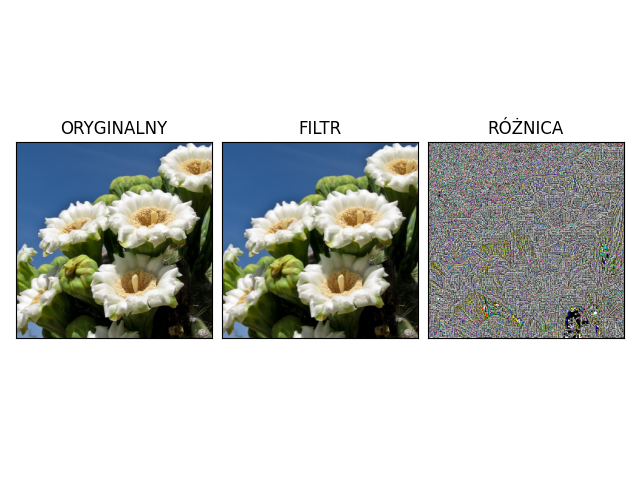
\includegraphics[scale=0.7]{images/nn_k1_p8.png}
    \\ \small Obraz 3. po interpolacji najbliższego sąsiada, 
    $k=1$, $p=8$.

    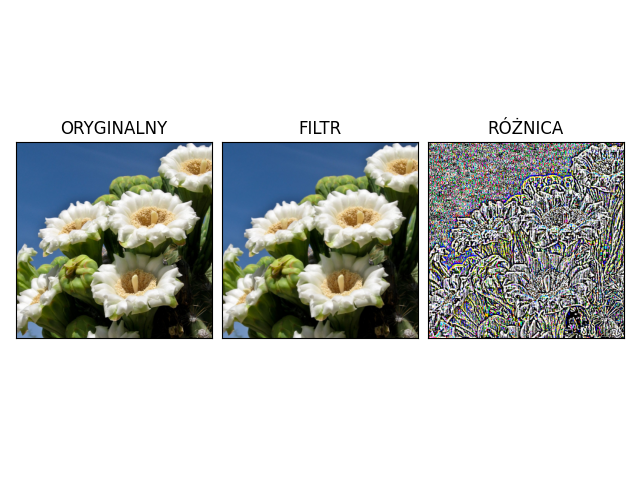
\includegraphics[scale=0.7]{images/lin_k1_p7.png}
    \\ \small Obraz 3. po interpolacji linearnej, 
    $k=1$, $p=7$.

    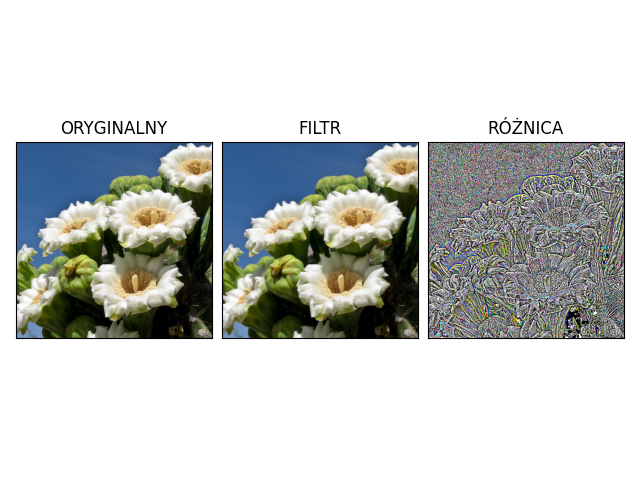
\includegraphics[scale=0.7]{images/lin_k1_p8.png}
    \\ \small Obraz 4. po interpolacji linearnej,
    $k=1$, $p=8$.

    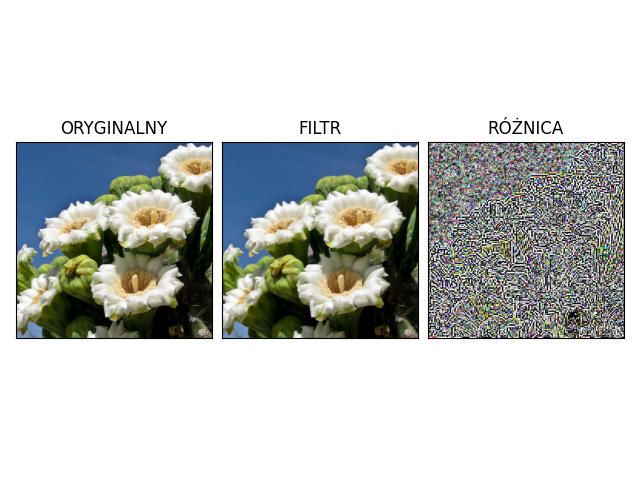
\includegraphics[scale=0.7]{images/keys_k1_p7.png}
    \\ \small Obraz 5. po interpolacji funkcją Keysa,
    $k=1$, $p=7$.

    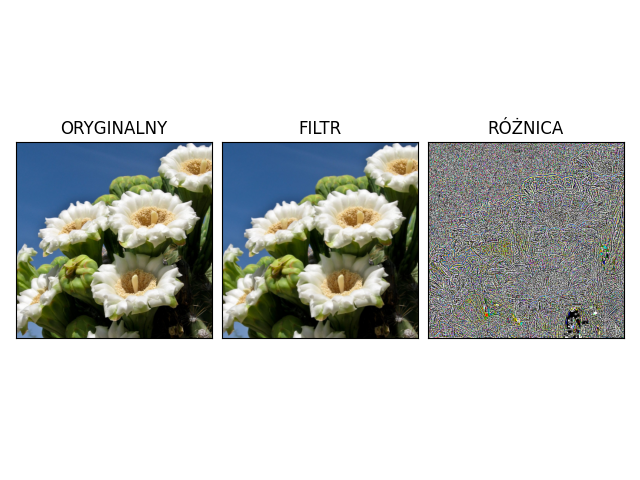
\includegraphics[scale=0.7]{images/keys_k1_p8.png}
    \\ \small Obraz 6. po interpolacji funkcją Keysa,
    $k=1$, $p=8$.

    %%%%%%%%%%%%%%%%%%%%%%%%%%%%%%%%%%%%%%%%%%%%%%%%%
    %
    % k = 3
    %

    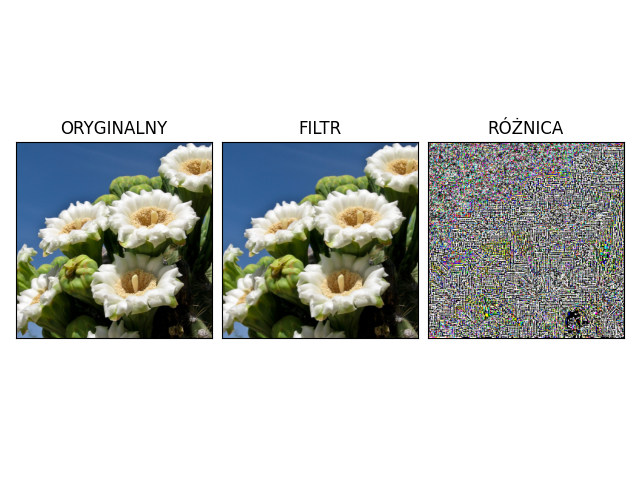
\includegraphics[scale=0.7]{images/nn_k3_p7.png}
    \\ \small Obraz 7. po interpolacji najbliższego sąsiada, 
    $k=3$, $p=7$.

    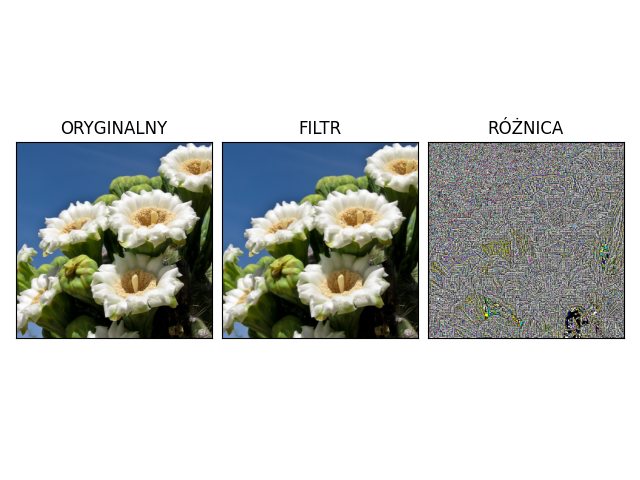
\includegraphics[scale=0.7]{images/nn_k3_p8.png}
    \\ \small Obraz 8. po interpolacji najbliższego sąsiada, 
    $k=3$, $p=8$.

    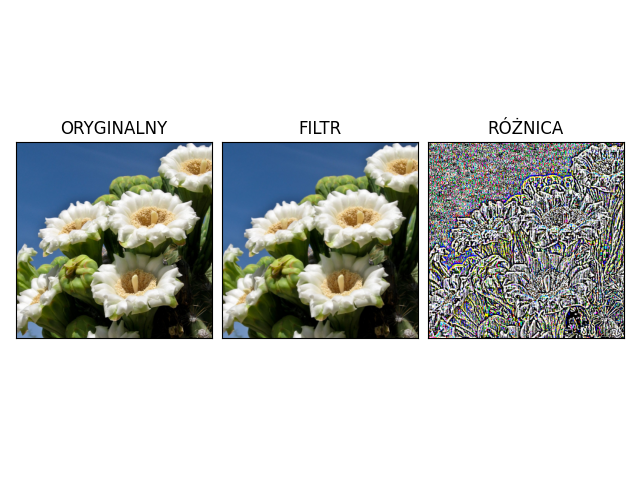
\includegraphics[scale=0.7]{images/lin_k3_p7.png}
    \\ \small Obraz 9. po interpolacji linearnej, 
    $k=3$, $p=7$.

    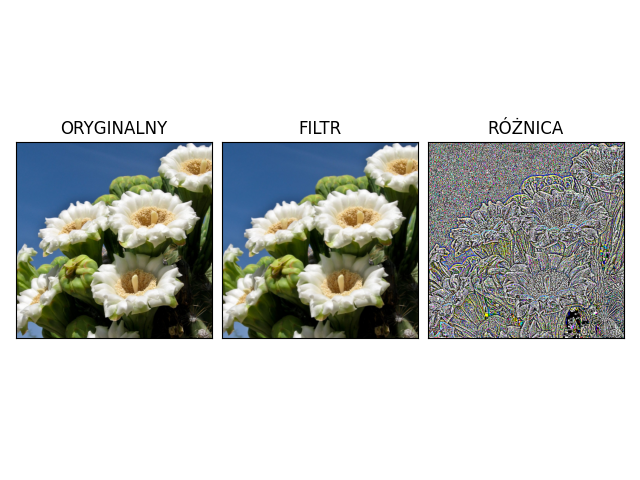
\includegraphics[scale=0.7]{images/lin_k3_p8.png}
    \\ \small Obraz 10. po interpolacji linearnej,
    $k=3$, $p=8$.

    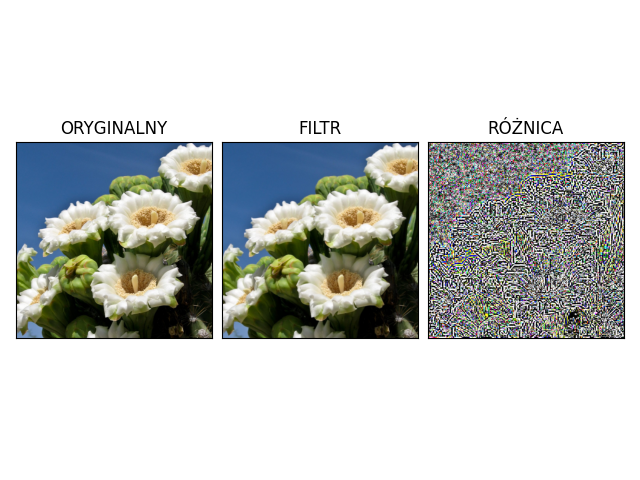
\includegraphics[scale=0.7]{images/keys_k3_p7.png}
    \\ \small Obraz 11. po interpolacji funkcją Keysa,
    $k=3$, $p=7$.

    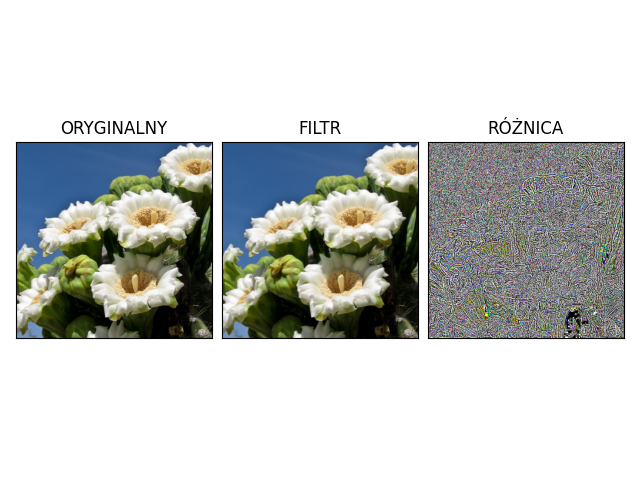
\includegraphics[scale=0.7]{images/keys_k3_p8.png}
    \\ \small Obraz 12. po interpolacji funkcją Keysa,
    $k=3$, $p=8$.

    %%%%%%%%%%%%%%%%%%%%%%%%%%%%%%%%%%%%%%%%%%%%
    %
    % POPRZEDNIE LABY
    %

    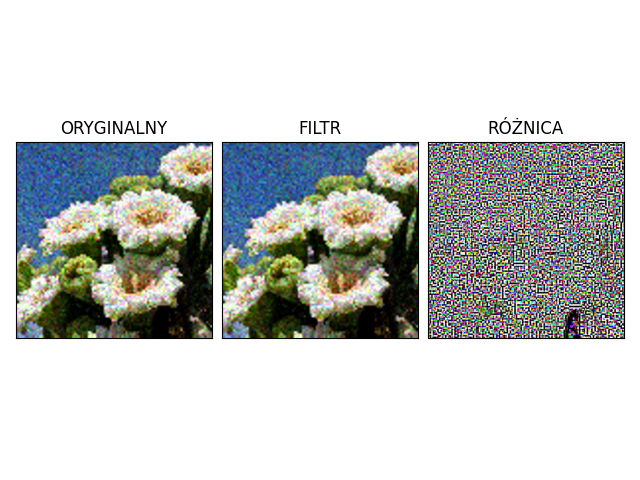
\includegraphics[scale=0.7]{images/keys_poisson1x_k1_p7.png}
    \\ \small Obraz 13. po interpolacji najbliższego sąsiada, 
    $k=1$, $p=7$, $\lambda=1$.

    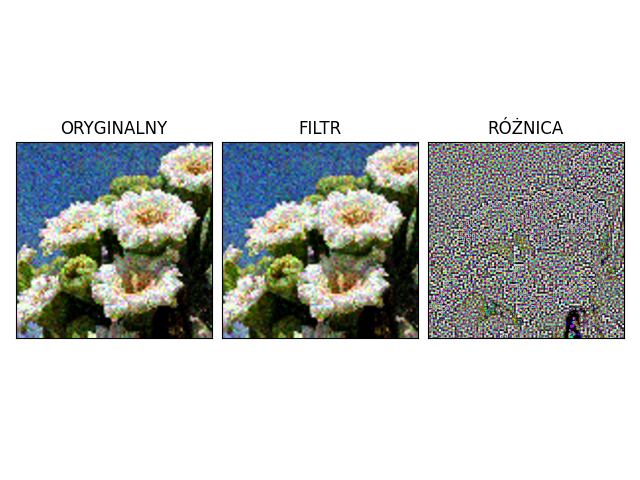
\includegraphics[scale=0.7]{images/keys_poisson1x_k1_p8.png}
    \\ \small Obraz 14. po interpolacji najbliższego sąsiada, 
    $k=1$, $p=8$, $\lambda=1$.

    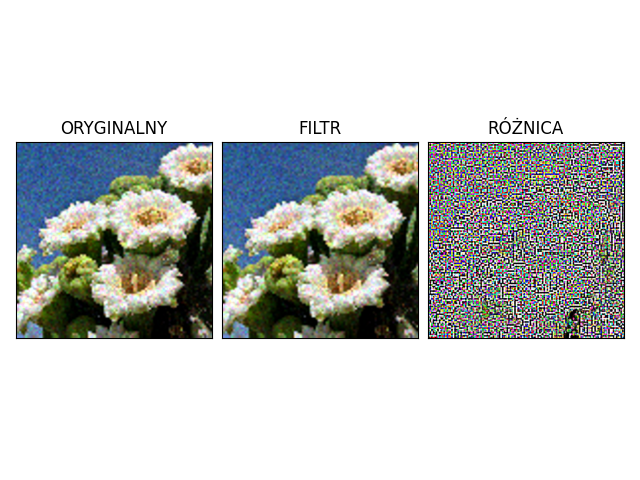
\includegraphics[scale=0.7]{images/keys_poisson4x_k1_p7.png}
    \\ \small Obraz 15. po interpolacji linearnej, 
    $k=1$, $p=7$, $\lambda=4$.

    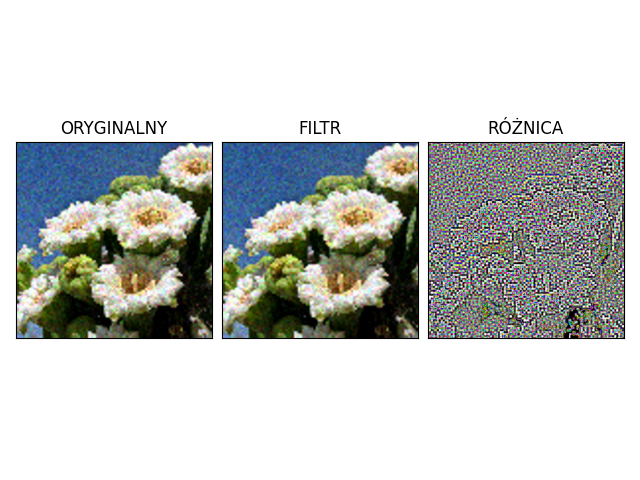
\includegraphics[scale=0.7]{images/keys_poisson4x_k1_p8.png}
    \\ \small Obraz 16. po interpolacji linearnej,
    $k=1$, $p=8$, $\lambda=4$.

    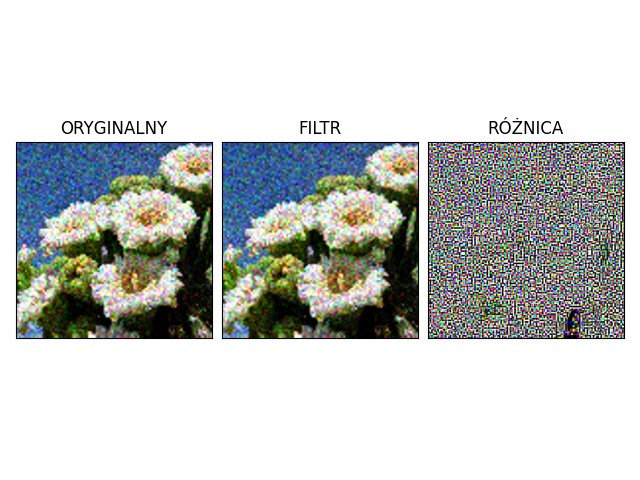
\includegraphics[scale=0.7]{images/keys_poisson16x_k1_p7.png}
    \\ \small Obraz 17. po interpolacji funkcją Keysa,
    $k=1$, $p=7$, $\lambda=16$.

    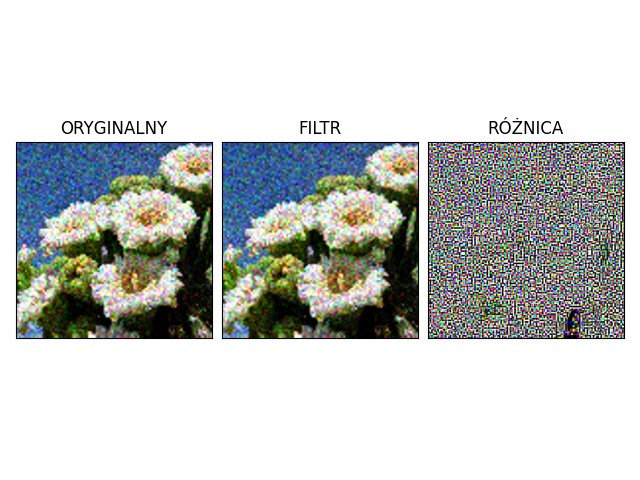
\includegraphics[scale=0.7]{images/keys_poisson16x_k1_p7.png}
    \\ \small Obraz 18. po interpolacji funkcją Keysa,
    $k=1$, $p=8$, $\lambda=16$.


\end{center}

\newpage
\section{Wnioski}


\begin{center}
    \vspace{0.2cm}
    %Subiektywnie patrząc, najlepiej w 
    %obu przypadkach wypadła interpolacja liniowa, dla $\lambda=4$ 
    %funkcja Keysa wypadła tylko odrobinę lepiej mając nieco mniejsze 
    %błędy MSE oraz MAE, ale wadą w przypadku użycia interpolacji linearnej
    %jest spore rozmazanie końcowego obrazu. Można także zauwayżyć zależność
    %MSE oraz MAE od $\lambda$ (średnia liczba zarejstrowanych fotonów)
    %- widać, że skala obu błędów powiększa się.

    Subiektywnie patrząc, najlepiej pod względem MSE oraz MAE w obu
    przypadkach $k=1$ oraz $k=3$, wypadła funkcja Keys'a
    zostawiając daleko w tyle
    interpolację liniową oraz najbliższego sąsiada.
    %Dla funkcji Keys'a najlepszą wartością było $k=1$ 
    %dla obu wartości $p$.

    \begin{itemize}
        \item Przy zastosowaniu większego $k$ 
        usuwamy więcej szumów jednocześnie tracąc więćej szczegółów,
        \item Dla funkcji Keys'a dla obrazu oryginalnego 
        oraz obrazów z poprzednich zajęć, wartość $k=1$ wartościo wyszła
        najlepiej,
        \item Wraz z większą ilością $k$, filtrowanie zajmuję więcej czasu,
        dla $k=1$ oraz $k=3$ jest to około 15-30 sekund, dla $k=5$ jest to już
        70 sekund, a dla $k=7$ ponad 30 minut,
        \item Patrząc na obrazy uzyskane na poprzednich zajęciach można
        szczególnie zauważyć wygładzenie i usunięcie szumów poprzez filtr, 
        dobrym przykładem tego jest obraz 16.
    \end{itemize}


    \vspace{1.25cm}
    \begin{tabular}{|c|c|c|c|c|}
        % MSE - kwadratowy
        % MAE - absolutny
        \hline
        %
        & \multicolumn{4}{|c|}{$k=1$} \\ \hline
        & \multicolumn{2}{|c|}{$p=7$} & \multicolumn{2}{|c|}{$p=8$} \\ \hline
        %

        & MSE & MAE & MSE & MAE \\ \hline
        Naj. sąsiada 
        & 250,38 & 7,32 % p = 7 
        & 102,2 & 4,56 \\ \hline % p =8 
        %%%%%%%%%%%%%%%%%%%%%%%%%%%%%%%%%%%%%%%%%%%%
        Linearna 
        & 276,59 & 8,46 % p = 7
        & 95,05 & 4,64 \\ \hline % p = 8
        %%%%%%%%%%%%%%%%%%%%%%%%%%%%%%%%%%%%%%%%%%%%
        Keysa 
        & 139,61 & 5,88 % p =7 
        & 50,76 & 3,37 \\ \hline % p = 8

    \end{tabular}
    \vspace{0.2cm}
    \\ \small Tabela 1. przedstawiająca błędy MSE oraz MAE dla $k=1$.


    %%%%%%%%%%%%%%%%%%%%%%%%%%%%%%%%%%%%%%%%%%%%%%%%%%%%%%%%%%%%%%%%

    \vspace{0.25cm}
    \begin{tabular}{|c|c|c|c|c|}
        % MSE - kwadratowy
        % MAE - absolutny
        \hline
        %
        & \multicolumn{4}{|c|}{$k=3$} \\ \hline
        & \multicolumn{2}{|c|}{$p=7$} & \multicolumn{2}{|c|}{$p=8$} \\ \hline
        %

        & MSE & MAE & MSE & MAE \\ \hline
        Naj. sąsiada 
        & 249,62 & 7,32 % p = 7 
        & 102,03 & 4,57 \\ \hline % p =8 
        %%%%%%%%%%%%%%%%%%%%%%%%%%%%%%%%%%%%%%%%%%%%
        Linearna 
        & 276,24 & 8,46 % p = 7
        & 95,11 & 4,64 \\ \hline % p = 8
        %%%%%%%%%%%%%%%%%%%%%%%%%%%%%%%%%%%%%%%%%%%%
        Keysa 
        & 139,25 & 5,87 % p =7 
        & 50,89 & 3,38 \\ \hline % p = 8

    \end{tabular}
    \vspace{0.2cm}
    \\ \small Tabela 2. przedstawiająca błędy MSE oraz MAE dla $k=3$.


        %%%%%%%%%%%%%%%%%%%%%%%%%%%%%%%%%%%%%%%%%%%%%%%%%%%%%%%%%%%%%%%%

        \vspace{0.25cm}
        \begin{tabular}{|c|c|c|c|c|}
            % MSE - kwadratowy
            % MAE - absolutny
            \hline
            %
            & \multicolumn{4}{|c|}{$k=1$} \\ \hline
            & \multicolumn{2}{|c|}{$p=7$} & \multicolumn{2}{|c|}{$p=8$} \\ \hline
            %
    
            & MSE & MAE & MSE & MAE \\ \hline
            $\lambda = 1$ 
            & 35,09 & 3,98 % p = 7 
            & 3,28 & 1,3 \\ \hline % p =8 
            %%%%%%%%%%%%%%%%%%%%%%%%%%%%%%%%%%%%%%%%%%%%
            $\lambda = 4$ 
            & 21,22 & 3,07 % p = 7
            & 2,2 & 1,09 \\ \hline % p = 8
            %%%%%%%%%%%%%%%%%%%%%%%%%%%%%%%%%%%%%%%%%%%%
            $\lambda = 16$ 
            & 48,05 & 4,68 % p =7 
            & 4,27 & 1,47 \\ \hline % p = 8
    
        \end{tabular}
        \vspace{0.2cm}
        \\ \small Tabela 3. przedstawiająca błędy MSE oraz MAE 
        dla obrazów uzyskanych na poprzednich laboratoriach, funkcja Keys'a, $k=1$.
\end{center}

\end{document}